\documentclass[twoside]{article}

\usepackage{epsfig}
\usepackage{amsmath,amssymb}
\usepackage{array}
\usepackage{booktabs}
\usepackage{enumitem}
\usepackage{float}
\usepackage{graphicx}
\usepackage{hyperref}
\usepackage[protrusion=true,expansion=false]{microtype}
\usepackage{xcolor}
\usepackage{tikz}
\usetikzlibrary{arrows.meta,calc,decorations.pathreplacing,fit,matrix,positioning}

\setlength{\oddsidemargin}{0 in}
\setlength{\evensidemargin}{0 in}
\setlength{\topmargin}{-0.6 in}
\setlength{\textwidth}{6.5 in}
\setlength{\textheight}{8.5 in}
\setlength{\headsep}{0.75 in}
\setlength{\parindent}{0 in}
\setlength{\parskip}{0.1 in}
\flushbottom

\hypersetup{
  colorlinks=true,
  linkcolor=blue!50!black,
  urlcolor=blue!50!black,
  citecolor=blue!50!black
}

\setlist[itemize]{leftmargin=1.5em,itemsep=0.16em,topsep=0.18em}
\setlist[enumerate]{leftmargin=1.6em,itemsep=0.16em,topsep=0.18em}

\newcommand{\lecture}[3]{
  \pagestyle{myheadings}
  \thispagestyle{plain}
  \newpage
  \setcounter{page}{1}
  \noindent
  \begin{center}
  \framebox{
    \vbox{\vspace{2mm}
    \hbox to 6.28in { {\bf CSE 291A/DSC 291: Data Systems for Machine Learning, Spring 2026 \hfill} }
    \vspace{6mm}
    \hbox to 6.28in { {\Large \hfill #1 \hfill} }
    \vspace{6mm}
    \hbox to 6.28in {%
      \begin{minipage}[t]{1.65in}{\itshape Lecturer: #2}\end{minipage}%
      \hfill
      \begin{minipage}[t]{4.55in}
        \begin{flushright}
          {\itshape\scriptsize Scribes: #3}
        \end{flushright}
      \end{minipage}%
    }
    \vspace{2mm}}
  }
  \end{center}
  \markboth{#1}{#1}
  \vspace*{4mm}
}

\definecolor{prefill}{RGB}{30,116,180}
\definecolor{decode}{RGB}{44,160,44}
\definecolor{cache}{RGB}{214,126,44}
\definecolor{queue}{RGB}{96,96,96}
\definecolor{lightblue}{RGB}{227,241,252}
\definecolor{lightgreen}{RGB}{228,246,226}
\definecolor{lightorange}{RGB}{255,239,221}
\definecolor{lightgray}{RGB}{242,242,242}

\newcommand{\kv}{\mathrm{KV}}
\newcommand{\HBM}{\mathrm{HBM}}
\newcommand{\SRAM}{\mathrm{SRAM}}
\newcommand{\EOS}{\texttt{<EOS>}}

\begin{document}

\lecture{15: LLM Inference and Serving}{Hao Zhang}{Suraj Ranganath, Vaishak Menon, Arunima Anand, Jackson Wilke, Atharv Nair, Rishika Mundada, Anish Patnaik, Kris Dcosta, Ishan Jain}

\section{Recap: Prefill, Decode, and Batch Size}

The lecture began with a quick recap of last week's discussion of language model inference.  A request first goes through the \textbf{prefill phase}, which is the zeroth iteration: the system gets the user prompt and processes all tokens in the prompt in one pass.  After prefill, the system starts the \textbf{decoding phase}, which covers the remaining iterations until the request hits the maximum sequence length or the model emits an end-of-sequence token such as \EOS.

The prefill and decoding phases have different compute and memory characteristics.  During prefill, all tokens in the prompt are seen in one pass, so the computation looks similar to training.  During decoding, the system can only decode one token at a time.  In the tensor shapes from the previous lecture, this means the sequence dimension \(s\) degenerates to \(1\).  If \(s=1\) and the batch size \(b\) is also small, the GPU is basically handling vectors and cannot saturate all of its streaming multiprocessors.

The recap also revisited the KV Cache.  During decoding, the query of the current token attends to the previous keys and values in the context.  The KV Cache is not ephemeral like activations from one forward computation; it persists on GPU memory during the lifecycle of the request.  Its size grows with sequence length, and the inference-time dimension that matters most for serving is \(b\), the number of concurrent requests currently being handled.

\begin{figure}[h]
\centering
\resizebox{0.96\linewidth}{!}{%
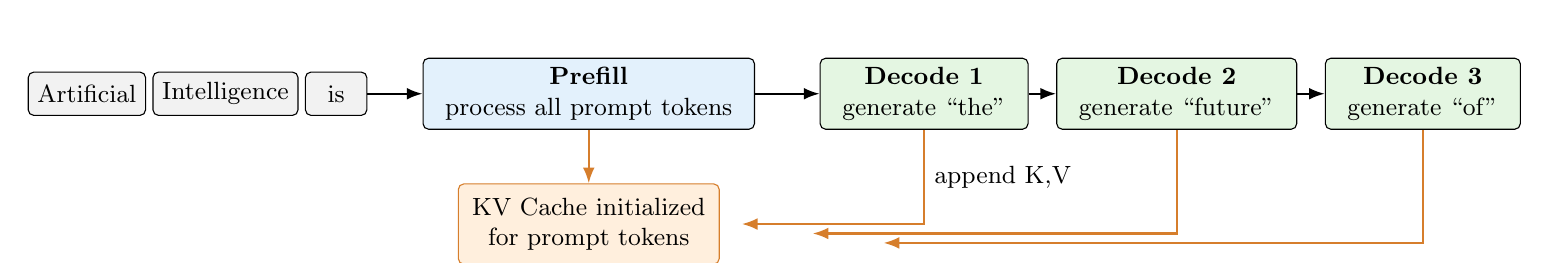
\begin{tikzpicture}[
  font=\small,
  box/.style={draw, rounded corners=2pt, minimum height=0.8cm, align=center, inner xsep=8pt},
  token/.style={draw, rounded corners=2pt, minimum height=0.55cm, minimum width=0.78cm, fill=lightgray},
  cachebox/.style={draw=cache, fill=lightorange, rounded corners=2pt, align=center, inner sep=5pt},
  arr/.style={-{Latex[length=2mm]}, thick}
]
\node[token] (a) at (0,0) {Artificial};
\node[token, right=0.08cm of a] (b) {Intelligence};
\node[token, right=0.08cm of b] (c) {is};
\node[box, fill=lightblue, right=0.7cm of c] (prefill) {\textbf{Prefill}\\process all prompt tokens};
\node[cachebox, below=0.68cm of prefill] (cache0) {KV Cache initialized\\for prompt tokens};
\node[box, fill=lightgreen, right=0.82cm of prefill] (dec1) {\textbf{Decode 1}\\generate ``the''};
\node[box, fill=lightgreen, right=0.35cm of dec1] (dec2) {\textbf{Decode 2}\\generate ``future''};
\node[box, fill=lightgreen, right=0.35cm of dec2] (dec3) {\textbf{Decode 3}\\generate ``of''};
\draw[arr] (c) -- (prefill);
\draw[arr] (prefill) -- (dec1);
\draw[arr] (dec1) -- (dec2);
\draw[arr] (dec2) -- (dec3);
\draw[arr, cache] (prefill) -- (cache0);
\draw[arr, cache] (dec1.south) |- ($(cache0.east)+(0.28,0.0)$) node[pos=0.25, right, black] {append K,V};
\draw[arr, cache] (dec2.south) |- ($(cache0.east)+(1.18,-0.12)$);
\draw[arr, cache] (dec3.south) |- ($(cache0.east)+(2.08,-0.24)$);
\end{tikzpicture}
}
\caption{One prefill pass processes the prompt, then decode generates one token per iteration.  The KV Cache stores per-layer keys and values so later decode steps do not recompute attention states for earlier tokens.}
\label{fig:prefill-decode}
\end{figure}

\section{Serving Versus Inference}

The lecture then distinguished two language-model inference scenarios.  The first scenario is \textbf{serving}: a hosted language model endpoint is listening to many users simultaneously.  Users submit requests at unknown times, so the traffic is online and dynamic.  The objective is throughput, because the provider wants to use the rented GPUs to serve as many users as possible.

The second scenario is \textbf{inference} in the narrower sense used in this part of lecture: the system is handling one request, or only a very small number of requests.  This is not online serving with many users.  In this case the objective is latency: the request should finish as fast as possible.

\begin{center}
\begin{tabular}{@{}p{0.22\linewidth}p{0.36\linewidth}p{0.34\linewidth}@{}}
\toprule
Regime & Setting & Main objective \\
\midrule
Serving & A hosted endpoint provides service to many users.  Requests arrive as online traffic, so arrival time and request content are dynamic. & Maximize throughput: serve as many users as possible with the available GPUs. \\
Inference & One request, or a very small number of requests, is being handled. & Minimize latency for those few requests. \\
\bottomrule
\end{tabular}
\end{center}

Mapping these two cases back to batch size, serving is the large-\(b\) case and inference is the small-\(b\) case, for example \(b=1\).  The rest of the lecture used this split to rethink the bottlenecks.

\section{Bottlenecks at Large and Small Batch Size}

\subsection{Large \(b\): online serving}

For large \(b\), the engine is handling many people submitting requests at the same time.  In prefill, the problem is that different prompts have different lengths.  The input shape is \((b,s,h)\), but every request in the batch may have a different \(s\).  One way to form a batch is to pad the shorter requests to the length of the longest request.  Padding works, but it wastes compute cycles on padded tokens.

For decode, different requests have different and unknown numbers of generated tokens.  A request may stop because it reaches the maximum sequence length, but most requests stop because the model emits \EOS.  When the model emits \EOS{} is only known at runtime, so the engine faces a dynamic termination problem.  During decode, \(s=1\) for each request, but \(b\) is large; therefore the computation is still GEMM rather than GEMV because the batch dimension and hidden dimension are both large.

On the memory side, each request needs its own KV Cache.  The KV Cache size grows with \(b\), so when \(b\) is large the system must allocate a lot of GPU memory to persist the KV Cache during the lifecycle of all active requests.  These three problems, different prompt lengths, dynamic termination, and KV Cache growth, are the key problems in a real serving system.

\subsection{\(b=1\): inference}

When \(b=1\), the prefill batching problem disappears because there is only one request.  The unknown generated-token problem still exists, but the main problem is decode.  During decode, both \(b=1\) and \(s=1\).  The operations degenerate to GEMV.  GEMV is easy for the GPU to compute, so compute is not the bottleneck.

The bottleneck is moving memory.  For every token and every matrix, the system moves data between memory levels such as HBM and SRAM.  This is what the lecture called being \textbf{memory bandwidth bound}.  In terms of arithmetic intensity,
\[
  \mathrm{AI} = \frac{\#\mathrm{ops}}{\#\mathrm{bytes}}.
\]
At \(b=1\), the numerator is small because there are very few FLOPs, while the denominator remains large because the model weights are large and still need to move through the memory hierarchy.  For KV Cache, the \(b=1\) case is simpler: there is only one request, so KV Cache memory is not the main bottleneck.

\subsection{Speculative decoding intuition}

Speculative decoding addresses the \(b=1\) problem.  During decoding, the system decodes one token, runs the model again on the next token, and repeats.  For each step, the model forwards one token through all layers, which requires moving model weights and activations between HBM and SRAM.  This is an algorithm constraint: the next token depends on the previous token.

The latency equation is
\[
  \mathrm{latency} = \mathrm{step\ latency} \times \#\mathrm{steps}.
\]
The step latency is dominated by memory movement, and the number of steps is the number of decoded tokens.  Speculative decoding tries to reduce the number of steps: instead of decoding one token per step, it tries to decode \(k\) tokens per step.  If the system can verify \(k\) tokens after moving the weights once, it amortizes the memory movement cost over those tokens.

The basic mechanism is to use a \textbf{draft model} to speculate a few tokens, then pass those tokens through the main model to verify them.  Tokens that match what the main model would have produced are accepted, and wrong tokens are rejected.  The lecture only gave this intuition because the main lecture focus was large-\(b\) serving.

\begin{figure}[H]
\centering
\resizebox{0.96\linewidth}{!}{%
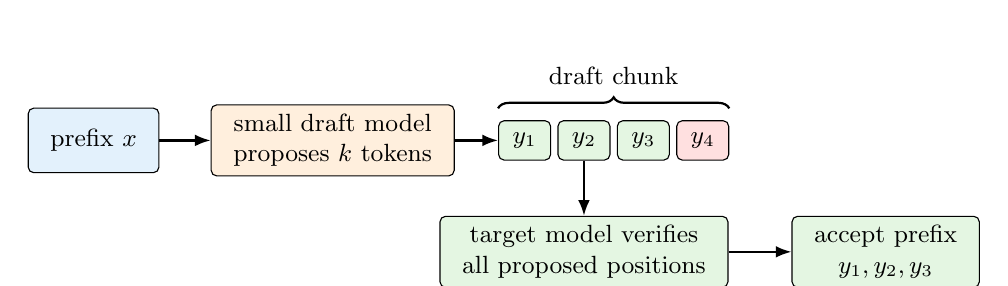
\begin{tikzpicture}[
  font=\small,
  stage/.style={draw, rounded corners=2pt, align=center, minimum height=0.82cm, inner xsep=8pt},
  tok/.style={draw, rounded corners=2pt, fill=lightgray, minimum width=0.66cm, minimum height=0.5cm},
  acc/.style={tok, fill=lightgreen},
  rej/.style={tok, fill=red!12},
  arr/.style={-{Latex[length=2mm]}, thick}
]
\node[stage, fill=lightblue] (prompt) {prefix \(x\)};
\node[stage, fill=lightorange, right=0.65cm of prompt] (draft) {small draft model\\proposes \(k\) tokens};
\node[acc, right=0.55cm of draft] (y1) {\(y_1\)};
\node[acc, right=0.08cm of y1] (y2) {\(y_2\)};
\node[acc, right=0.08cm of y2] (y3) {\(y_3\)};
\node[rej, right=0.08cm of y3] (y4) {\(y_4\)};
\node[stage, fill=lightgreen, below=0.7cm of y2] (verify) {target model verifies\\all proposed positions};
\node[stage, fill=lightgreen, right=0.8cm of verify] (accept) {accept prefix\\\(y_1,y_2,y_3\)};
\draw[arr] (prompt) -- (draft);
\draw[arr] (draft) -- (y1);
\draw[arr] (y2.south) -- (verify.north);
\draw[arr] (verify) -- (accept);
\draw[decorate, decoration={brace, amplitude=4pt}, thick]
  ($(y1.north west)+(0,0.15)$) -- ($(y4.north east)+(0,0.15)$)
  node[midway, above=5pt] {draft chunk};
\end{tikzpicture}
}
\caption{Speculative decoding trades extra draft-model work for fewer expensive target-model decode steps.  It is useful when target-model decode is memory-bandwidth bound and the draft acceptance rate is high.}
\label{fig:speculative}
\end{figure}

\section{Serving Techniques: Continuous Batching and PagedAttention}

After the small-\(b\) discussion, the lecture shifted back to large \(b\), which is the more complicated serving scenario.  The three problems were repeated: large batches have uneven sequence length, each request does not know when it will terminate, and the KV Cache grows with batch size.  The two notable optimizations introduced were \textbf{continuous batching} and \textbf{PagedAttention}.  This lecture finished continuous batching and only provided the motivation for PagedAttention.

\subsection{Static batching and its limitations}

The lecture next used a timeline view of text generation.  A single request starts with a yellow prefill segment, then produces blue decoded tokens one by one, and stops when the red \EOS{} token is emitted.  When there are many requests, the naive approach is \textbf{static batching}: group requests together, run their prefill together, and keep the batch fixed until all requests finish.

Static batching wastes work because requests finish at different iterations.  If \(S_1\) and \(S_3\) finish early but \(S_2\) continues to a later iteration, the early requests remain tied to the batch.  Their GPU slots cannot be reused immediately.  From the user's perspective, a completed answer may wait behind the longest sequence in the batch.  From the system's perspective, finished requests create idle capacity while new requests sit in a queue.

\begin{figure}[H]
\centering
\resizebox{0.92\linewidth}{!}{%
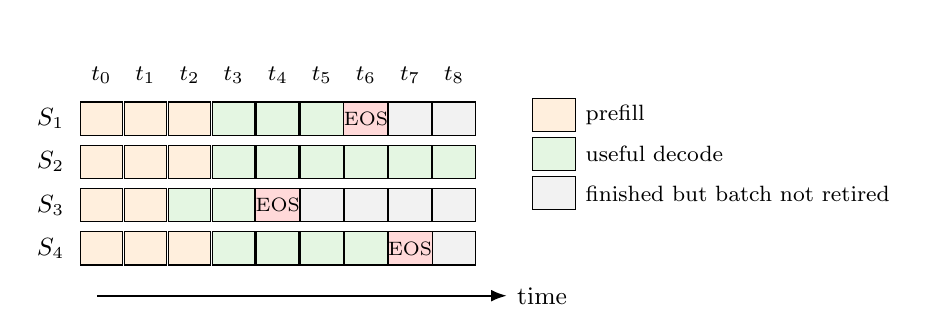
\begin{tikzpicture}[
  font=\small,
  cell/.style={draw, minimum width=0.54cm, minimum height=0.42cm, inner sep=0pt},
  pre/.style={cell, fill=lightorange},
  dec/.style={cell, fill=lightgreen},
  wait/.style={cell, fill=lightgray},
  eos/.style={cell, fill=red!15},
  axis/.style={-{Latex[length=2mm]}, thick}
]
\node[anchor=east] at (-0.35,0) {\(S_1\)};
\node[anchor=east] at (-0.35,-0.55) {\(S_2\)};
\node[anchor=east] at (-0.35,-1.10) {\(S_3\)};
\node[anchor=east] at (-0.35,-1.65) {\(S_4\)};
\foreach \x in {0,...,8} {
  \node[font=\footnotesize] at (\x*0.56,0.55) {\(t_{\x}\)};
}
\foreach \x in {0,1,2} \node[pre] at (\x*0.56,0) {};
\foreach \x in {3,4,5} \node[dec] at (\x*0.56,0) {};
\node[eos] at (6*0.56,0) {\scriptsize EOS};
\foreach \x in {7,8} \node[wait] at (\x*0.56,0) {};

\foreach \x in {0,1,2} \node[pre] at (\x*0.56,-0.55) {};
\foreach \x in {3,4,5,6,7,8} \node[dec] at (\x*0.56,-0.55) {};

\foreach \x in {0,1} \node[pre] at (\x*0.56,-1.10) {};
\foreach \x in {2,3} \node[dec] at (\x*0.56,-1.10) {};
\node[eos] at (4*0.56,-1.10) {\scriptsize EOS};
\foreach \x in {5,6,7,8} \node[wait] at (\x*0.56,-1.10) {};

\foreach \x in {0,1,2} \node[pre] at (\x*0.56,-1.65) {};
\foreach \x in {3,4,5,6} \node[dec] at (\x*0.56,-1.65) {};
\node[eos] at (7*0.56,-1.65) {\scriptsize EOS};
\node[wait] at (8*0.56,-1.65) {};
\draw[axis] (-0.05,-2.25) -- (5.15,-2.25) node[right] {time};
\node[pre, label=right:{\footnotesize prefill}] at (5.75,0.05) {};
\node[dec, label=right:{\footnotesize useful decode}] at (5.75,-0.45) {};
\node[wait, label=right:{\footnotesize finished but batch not retired}] at (5.75,-0.95) {};
\end{tikzpicture}
}
\caption{Static batching wastes iteration slots after shorter requests finish.  From the user's view, a request may have generated its answer but still wait for the longest request in the static batch.}
\label{fig:static-batching}
\end{figure}

This is the source of queueing latency.  Users expect their responses to begin quickly, but a static batch can make newly arrived requests wait until an existing batch drains.

\subsection{Continuous batching}

\textbf{Continuous batching} addresses this problem by dynamically forming the batch at the iteration level.  A modern language model engine has a CPU-side \textbf{request pool}, which listens to user requests, and a GPU-side \textbf{execution engine}, which runs the active requests.  In the lecture example, the execution engine has maximum serving batch size 3.

Suppose \(R_1\) is ``optimizing ML systems'' and \(R_2\) is ``LLM serving is''.  The request pool sees that the execution engine is idle and pushes both requests through.  Iteration 1 is prefill.  If the prompt lengths are different, padding would waste compute; instead, the engine breaks the transformer computation into sequence-dependent and token-dependent operations.

The attention softmax, \(\mathrm{softmax}(QK^T/\sqrt{d})\), is sequence-dependent because a token attends to previous tokens in the same sequence.  In contrast, the \(Q/K/V\) projections, output projection, RMSNorm, SwiGLU, MLP, and similar operations are token-level operations.  They take one token's hidden representation and apply a transformation to that token's vector.  For token-level operations, the engine can concatenate all real tokens from all requests into one big batch of shape \((\mathrm{total\ tokens}, h)\), avoiding padding.

\begin{figure}[H]
\centering
\resizebox{\linewidth}{!}{%
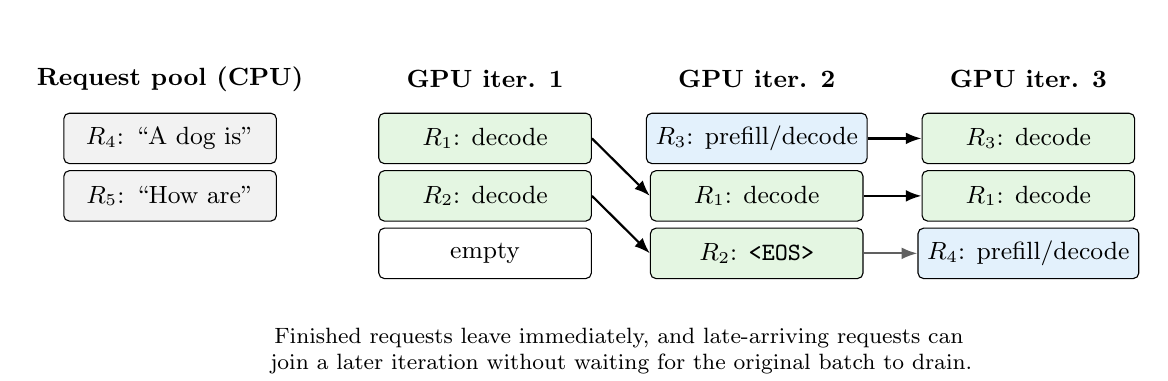
\begin{tikzpicture}[
  font=\small,
  slot/.style={draw, rounded corners=2pt, minimum width=2.7cm, minimum height=0.64cm, align=center},
  header/.style={font=\small\bfseries},
  arr/.style={-{Latex[length=2mm]}, thick}
]
\node[header] at (0,0.4) {Request pool (CPU)};
\node[slot, fill=lightgray] (q1) at (0,-0.35) {\(R_4\): ``A dog is''};
\node[slot, fill=lightgray] (q2) at (0,-1.08) {\(R_5\): ``How are''};

\node[header] at (4.0,0.4) {GPU iter. 1};
\node[slot, fill=lightgreen] (i1a) at (4.0,-0.35) {\(R_1\): decode};
\node[slot, fill=lightgreen] (i1b) at (4.0,-1.08) {\(R_2\): decode};
\node[slot, fill=white] (i1c) at (4.0,-1.81) {empty};

\node[header] at (7.45,0.4) {GPU iter. 2};
\node[slot, fill=lightblue] (i2a) at (7.45,-0.35) {\(R_3\): prefill/decode};
\node[slot, fill=lightgreen] (i2b) at (7.45,-1.08) {\(R_1\): decode};
\node[slot, fill=lightgreen] (i2c) at (7.45,-1.81) {\(R_2\): \EOS};

\node[header] at (10.9,0.4) {GPU iter. 3};
\node[slot, fill=lightgreen] (i3a) at (10.9,-0.35) {\(R_3\): decode};
\node[slot, fill=lightgreen] (i3b) at (10.9,-1.08) {\(R_1\): decode};
\node[slot, fill=lightblue] (i3c) at (10.9,-1.81) {\(R_4\): prefill/decode};

\draw[arr] (i1a.east) -- (i2b.west);
\draw[arr] (i1b.east) -- (i2c.west);
\draw[arr] (i2b.east) -- (i3b.west);
\draw[arr] (i2a.east) -- (i3a.west);
\draw[arr, queue] (i2c.east) -- (i3c.west);
\node[align=center, font=\footnotesize, text width=10.5cm] at (5.7,-3.05)
{Finished requests leave immediately, and late-arriving requests can join a later iteration without waiting for the original batch to drain.};
\end{tikzpicture}
}
\caption{Continuous batching follows the lecture's example: early exits and late arrivals are handled at iteration granularity.  The exact scheduler can be FIFO or more sophisticated, but the batch is not fixed for the lifetime of a request.}
\label{fig:continuous-batching}
\end{figure}

After prefill, \(R_1\) and \(R_2\) start decoding.  Each request contributes one decode token, so token-level operations can again be batched.  The attention part is harder because the new token from each request may attend to a different KV Cache length.  Earlier systems often issued separate attention kernels for these cases, which was acceptable because MLP-like work dominated much of the runtime.  More recent systems use variable-length attention kernels so that attention across different sequence lengths can also be batched.

When a later request such as \(R_3\) arrives, continuous batching can admit it at the iteration level instead of waiting for the old requests to finish.  The lecture used first-come-first-served, so the earliest waiting request enters first.  This creates the third case: batching prefill and decode together.  The same principle applies: issue attention work according to the sequence-dependent structure, and batch token-level operations across all tokens.  When a request emits \EOS, continuous batching lets it immediately exit the execution engine.

The mechanism gives three important abilities:
\begin{itemize}
  \item early-finished requests can leave immediately instead of waiting for the longest request;
  \item late-arriving requests can start as soon as capacity appears;
  \item prefill work for new requests can be batched with decode work for old requests.
\end{itemize}

The exact policy for choosing the next request is a scheduling problem.  The lecture used FCFS for simplicity, but emphasized that there is room for better scheduling policies.  The key mechanism is that the batch is dynamic: requests can join or exit at every iteration, reducing queueing time and improving GPU utilization.

Continuous batching also explains why modern hosted LLM services can stream tokens independently to different users.  Each request can return its own tokens as they are produced even though many requests share the same GPU iterations.

\subsection{Batching requests with different lengths}

Continuous batching is only useful if the model can process requests with different sequence lengths efficiently.  The key observation is the same as above: transformer operations fall into two groups.

\textbf{Sequence-dependent operations} need sequence boundaries and attention history.  The softmax attention computation \( \mathrm{softmax}(QK^T/\sqrt{d})V \) depends on which previous tokens belong to the same request.  During decode, each new query token may attend to a different KV Cache length.

\textbf{Token-dependent operations} do not fundamentally care which sequence a token came from.  RMSNorm, \(Q/K/V\) projections, output projections, MLPs, SwiGLU, and many MoE feed-forward computations apply the same transformation to each token representation.  For these operations, the system can collapse the sequence dimension:
\[
  (b, s, h) \quad \longrightarrow \quad
  \left(\sum_i s_i, h\right).
\]
This creates one dense batch of real tokens and avoids padding short prompts to the longest prompt.

This decomposition handles the three continuous-batching cases:
\begin{itemize}
  \item \textbf{Prefill with prefill:} prompts have different lengths; token-wise work is flattened, while attention respects sequence boundaries.
  \item \textbf{Decode with decode:} each request contributes one query token, but those tokens attend to KV Cache entries of different lengths.
  \item \textbf{Prefill with decode:} new prompts and ongoing decode tokens share token-wise kernels, while attention kernels handle different phases.
\end{itemize}

If the system simply forces every request into the same shape, the usual result is padding and wasted compute on padded tokens.  Serving systems instead form batches at the iteration level and break down the transformer into sequence-relevant and token-relevant operations.  For large models at moderate context lengths, this is effective because MLP-like work often dominates runtime.  The lecture gave the rule of thumb that attention may be around 20--30 percent of compute while MLP/projection work may be 70--80 percent.  At very long context length, attention can become the majority of the work, so kernels that can batch tokens attending to different sequence lengths become more important.

Recent systems increasingly batch the attention part too.  Variable-length attention batching and online softmax are now often written together into one GPU kernel.  The high-level serving engine decides scheduling and memory layout; optimized kernels make attention over different sequence lengths fast enough to keep the accelerator busy.

\begin{figure}[H]
\centering
\resizebox{0.96\linewidth}{!}{%
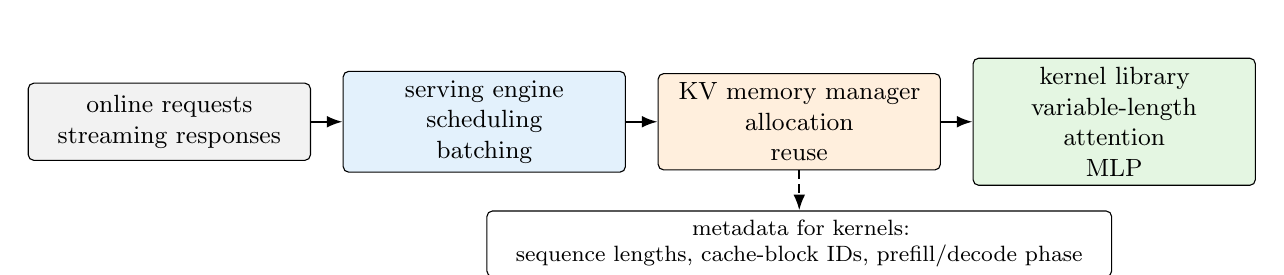
\begin{tikzpicture}[
  font=\small,
  layer/.style={draw, rounded corners=2pt, align=center, minimum height=0.98cm, text width=3.35cm},
  meta/.style={draw, rounded corners=2pt, align=center, font=\footnotesize, text width=7.7cm, fill=white},
  arr/.style={-{Latex[length=2mm]}, thick},
  metaarr/.style={-{Latex[length=2mm]}, thick, densely dashed}
]
\node[layer, fill=lightgray] (api) at (0,0) {online requests\\streaming responses};
\node[layer, fill=lightblue] (sched) at (4.0,0) {serving engine\\scheduling\\batching};
\node[layer, fill=lightorange] (mem) at (8.0,0) {KV memory manager\\allocation\\reuse};
\node[layer, fill=lightgreen] (kern) at (12.0,0) {kernel library\\variable-length attention\\MLP};
\node[meta] (meta) at (8.0,-1.55) {metadata for kernels:\\sequence lengths, cache-block IDs, prefill/decode phase};
\draw[arr] (api) -- (sched);
\draw[arr] (sched) -- (mem);
\draw[arr] (mem) -- (kern);
\draw[metaarr] (mem.south) -- (meta.north);
\end{tikzpicture}
}
\caption{Modern serving stacks split responsibilities.  The scheduler decides which requests run; the memory manager decides where KV entries live; optimized kernel libraries execute token-wise and variable-length attention work using the metadata supplied by the engine.}
\label{fig:serving-stack}
\end{figure}

\section{KV Cache and Motivation for PagedAttention}

After continuous batching, the lecture started the KV Cache section and used it to motivate PagedAttention.  The KV Cache stores the key and value vectors for each token at each layer.  For every token, there is one key vector and one value vector; every layer has its own attention, so every layer has its own KV Cache.  Ignoring implementation layout details, the cache size for active requests is approximately
\[
  M_{\kv}
  \approx
  2 \cdot L \cdot n_{\kv} \cdot d_{\mathrm{head}} \cdot a
  \cdot
  \sum_{r \in \mathrm{active}} T_r,
\]
where the factor of 2 is for keys and values, \(L\) is the number of layers, \(n_{\kv}\) is the number of KV heads, \(d_{\mathrm{head}}\) is the head dimension, \(a\) is bytes per element, and \(T_r\) is the cached token count for request \(r\).  The important dependence is on total active tokens.

From a systems perspective, the word ``cache'' is imperfect here.  In rigorous systems literature, a cache is useful when memory accesses hit, and the hit rate is not guaranteed.  For language model decoding, every new token attends to the previous keys and values, so the hit rate is effectively 100 percent during the request lifetime.  The lecture described this as a working set rather than a cache.  The size dynamically grows and shrinks: every decoded token appends a new entry, and when a request emits \EOS{} the engine can delete that request's KV Cache.

The lecture used an A100 40GB example to show why this matters.  A 13B model in BF16 needs roughly 26GB just for parameters, about 65 percent of the GPU memory.  Suppose about 1GB is reserved for ephemeral activations during forward computation.  That leaves roughly 13GB for the KV Cache of all concurrent requests.

\begin{figure}[H]
\centering
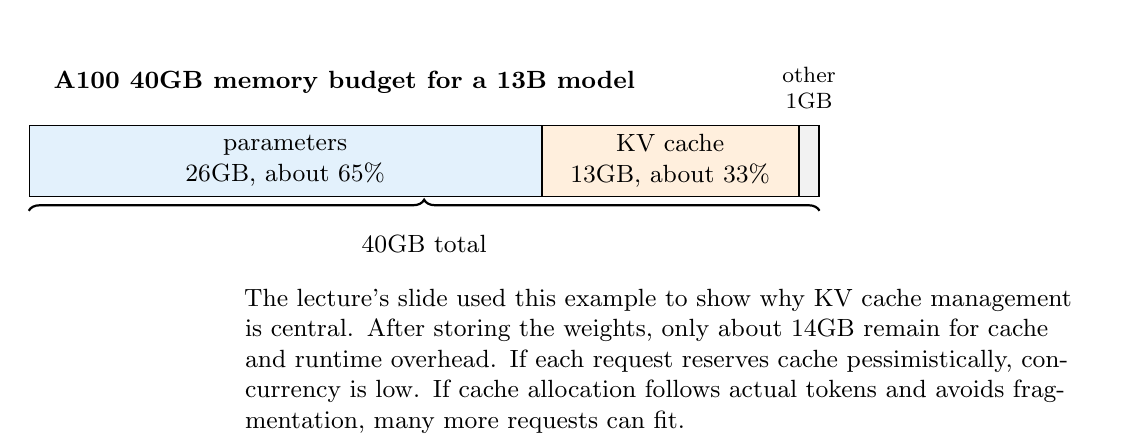
\begin{tikzpicture}[
  font=\small,
  mem/.style={draw, minimum height=0.9cm, align=center},
  label/.style={font=\small\bfseries}
]
\node[label] at (4.0,1.0) {A100 40GB memory budget for a 13B model};
\node[mem, fill=lightblue, minimum width=6.5cm] (param) at (3.25,0) {parameters\\26GB, about 65\%};
\node[mem, fill=lightorange, minimum width=3.25cm, right=0cm of param] (kv) {KV cache\\13GB, about 33\%};
\node[mem, fill=lightgray, minimum width=0.25cm, right=0cm of kv] (other) {};
\node[above=0.08cm of other, font=\footnotesize, align=center] {other\\1GB};
\draw[decorate, decoration={brace, amplitude=4pt}, thick]
  ($(param.south west)+(0,-0.18)$) -- ($(other.south east)+(0,-0.18)$)
  node[midway, below=5pt] {40GB total};
\node[align=left, text width=10.8cm, below=1.05cm of kv] {
The lecture's slide used this example to show why KV cache management is central.  After storing the weights, only about 14GB remain for cache and runtime overhead.  If each request reserves cache pessimistically, concurrency is low.  If cache allocation follows actual tokens and avoids fragmentation, many more requests can fit.
};
\end{tikzpicture}
\caption{In the 13B-on-A100 example, parameters dominate memory, but the remaining capacity is quickly consumed by KV cache.}
\label{fig:kv-memory}
\end{figure}

The throughput point is that batch size also controls how many streaming multiprocessors can be kept busy.  At small batch sizes the GPU is still hungry for more requests.  If the engine can accommodate a larger batch size under the same GPU memory limit, it can process more requests per unit time.

\begin{figure}[H]
\centering
\resizebox{0.92\linewidth}{!}{%
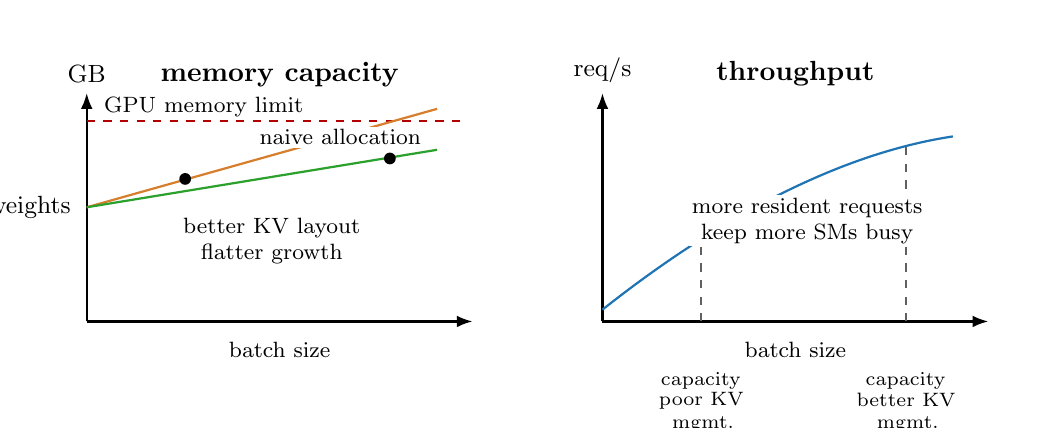
\begin{tikzpicture}[
  font=\small,
  axis/.style={-{Latex[length=2mm]}, thick},
  curve/.style={thick},
  dashedline/.style={dashed, thick},
  point/.style={circle, fill=black, inner sep=1.5pt}
]
\path[use as bounding box] (-0.75,-1.38) rectangle (11.85,3.35);
% Left plot: memory capacity
\node[font=\bfseries] at (2.45,3.13) {memory capacity};
\draw[axis] (0,0) -- (4.9,0);
\draw[axis] (0,0) -- (0,2.9) node[above] {GB};
\node[font=\footnotesize] at (2.45,-0.36) {batch size};
\draw[dashedline, red!70!black] (0,2.55) -- (4.75,2.55);
\node[font=\footnotesize, anchor=south west, fill=white, inner sep=1pt] at (0.18,2.56) {GPU memory limit};
\draw[curve, cache] (0,1.45) -- (4.45,2.70);
\draw[curve, decode] (0,1.45) -- (4.45,2.18);
\node[point] at (1.25,1.81) {};
\node[point] at (3.85,2.07) {};
\node[anchor=east] at (-0.08,1.45) {weights};
\node[align=center, font=\footnotesize, fill=white, inner sep=1pt] at (2.35,1.02) {better KV layout\\flatter growth};
\node[align=center, font=\footnotesize, fill=white, inner sep=1pt] at (3.22,2.34) {naive allocation};

% Right plot: throughput
\begin{scope}[xshift=6.55cm]
\node[font=\bfseries] at (2.45,3.15) {throughput};
\draw[axis] (0,0) -- (4.9,0);
\draw[axis] (0,0) -- (0,2.9) node[above] {req/s};
\node[font=\footnotesize] at (2.45,-0.36) {batch size};
\draw[curve, prefill] (0,0.15) .. controls (1.2,1.1) and (2.8,2.1) .. (4.45,2.35);
\draw[dashedline, queue] (1.25,0) -- (1.25,1.08);
\draw[dashedline, queue] (3.85,0) -- (3.85,2.25);
\node[font=\scriptsize, anchor=north] at (1.25,-0.52) {capacity};
\node[align=center, font=\scriptsize, text width=1.55cm, anchor=north] at (1.25,-0.78) {poor KV\\mgmt.};
\node[font=\scriptsize, anchor=north] at (3.85,-0.52) {capacity};
\node[align=center, font=\scriptsize, text width=1.55cm, anchor=north] at (3.85,-0.78) {better KV\\mgmt.};
\node[font=\footnotesize, align=center, fill=white, inner sep=1pt] at (2.60,1.28) {more resident requests\\keep more SMs busy};
\end{scope}
\end{tikzpicture}
}
\caption{KV-cache management links memory capacity to throughput.  If cache allocation grows too fast with batch size, the server hits the memory wall before the GPU reaches its useful throughput region.}
\label{fig:kv-throughput}
\end{figure}

If KV Cache management is inefficient, the system becomes \textbf{memory capacity bound}.  Memory fills up, so the server cannot accommodate more requests, and many GPU SMs sit idle.  If KV Cache is managed more carefully, the same GPU memory can hold more concurrent requests and the server can better use the GPU.

This motivates PagedAttention and vLLM.  The lecture only introduced why it is needed: existing systems can waste KV Cache memory; the next lecture explains how to fix that.

The lecture also answered a question about repeated prefixes.  If incoming requests share a long prefix, the server can reuse the previously computed KV entries for that prefix rather than recomputing and storing duplicate copies.  This is called prefix caching; RadixAttention is one example of organizing shared prefixes with a radix-tree-like structure over tokens.  Prefix caching is separate from continuous batching, but both aim to avoid wasting compute and memory on work that is not useful.

\section{Takeaways}

The main split is between small-batch latency optimization and large-batch serving throughput.  In the \(b=1\) regime, decode is memory-bandwidth bound because both \(b\) and \(s\) are 1; speculative decoding tries to reduce the number of expensive target-model steps.  In the large-\(b\) regime, the hard problems are requests with different sequence lengths, dynamic termination, queueing latency, and KV Cache memory growth.

Continuous batching addresses queueing and utilization by allowing requests to enter and leave at every iteration.  Its implementation depends on separating token-wise operations from sequence-dependent attention.  KV Cache management addresses the memory side: the cache grows with active tokens, so memory layout determines how many concurrent requests can fit on the GPU.  Together, continuous batching and efficient KV Cache management are core ingredients of high-throughput LLM serving.

\end{document}
